\documentclass{beamer}
\usepackage{amsmath, amssymb}
\usepackage{graphicx}

\title{Online cassification of ArXiv papers based on your preferences }

\author{Steven Delong and Joseph McDonald}


\begin{document}
\maketitle


\begin{frame}
  \frametitle{Goals}
  Wanted to create a tool to learn an individual's preferences for ArXiv articles.
\begin{itemize}
\item New articles added every day, we want to predict whether they are interesting and learn from them.
\item Natural setting for online learning.
\item Traditional online learning algorithms would ask for a label for every paper rendering them useless. Can we get away with asking for less of the articles that are uninteresting.
\end{itemize}


\end{frame}


\begin{frame}
\frametitle{Method}
\begin{itemize}
\item Start: simple perceptron and bag-of-words model.
\item Update always when  $\hat{y} = 1$, and with probability $p$ if $\hat{y} = -1$.
\item Can show that this achieves a bound on mistakes in expectation similar to normal perceptron $\mathbb{E}[M] \leq \frac{1}{p}\frac{r^2}{\rho^2}$.
\item Much weaker bound, but requires less ``work'' from the user.
\item Intuitively, maybe we should look at more of the $\hat{y} = -1$ observations when we're less sure of the algorithm.
\end{itemize}
\end{frame}

\begin{frame}
  \frametitle{Idea: Variable $p$}
 
\begin{itemize}
\item Start with $p = 1$, increase $p$ on false negatives, decrease $p$ on correct negative predictions.
\item Never reduce $p$ below some value $p_\min$. 
\item Set $p = p + \gamma_1(1 - p)$ when we're wrong, and $p = p - \gamma_2(p - p_\min)$ when correct.
\item Can show the same bound holds as in the constant $p$ case, using
  $p = p_\min$. $\mathbb{E}[M] \leq \frac{1}{p_{\min}}\frac{r^2}{\rho^2}$.
\end{itemize}
\end{frame}

\begin{frame}
\frametitle{Results}
We each labeled several articles, shuffled their order, and then
tested several online learning algorithms on them.  We measured recall
and number of labels used by the algorithm when $\hat{y} = -1$.
\begin{figure}
\centering
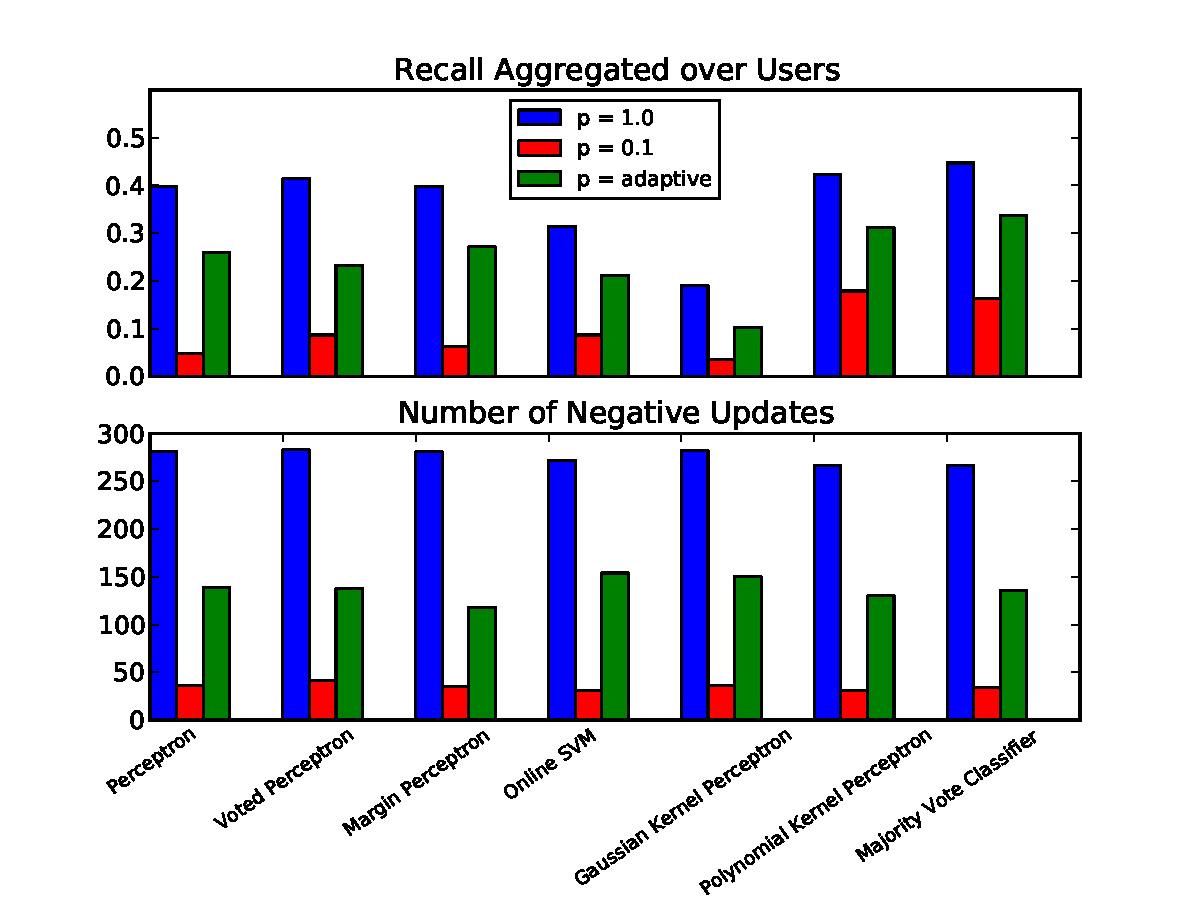
\includegraphics[width=0.7\textwidth]{EveryoneRecallPaper.pdf}
\end{figure}
\end{frame}


\begin{frame}
\frametitle{Conclusions}
\begin{itemize}
\item The modified algorithms perform reasonably well while requiring less labels.
\item We obtained bounds on  $\mathbb{E}[M]$ for the modified perceptron algorithms.
\item In the future: Better bounds on adaptive $p$, tune adaptive $p$, explore other features and algorithms.
\item Code available at www.github.com/skwaap/fml-arxiv.
\end{itemize}
\end{frame}



\end{document}  


